%% Chapter 14: Lead-Lag Compensation
%% IEEE-formatted Control Systems Textbook
%% Self-contained chapter with complete derivations and practical experiments

\chapter{Lead-Lag Compensation}
\label{ch:lead_lag}

\section*{Chapter Overview}
\addcontentsline{toc}{section}{Chapter Overview}

This chapter introduces lead and lag compensation---powerful frequency-domain design techniques that extend beyond simple PID control. We begin with the historical context of World War II fire control systems, where engineers faced the challenge of tracking fast-moving targets with unprecedented accuracy. This military necessity drove the development of phase-shaping networks that could boost system performance precisely where needed. Today, these techniques remain essential for systems requiring precise control over bandwidth and stability margins.

%% ============================================================================
%% SECTION 1: HISTORICAL MOTIVATION
%% ============================================================================
\section{Historical Motivation: From Anti-Aircraft Guns to Modern Servos}
\label{sec:lead_lag_history}

\begin{historicalbox}[The Fire Control Problem of World War II]
The development of lead-lag compensation is inextricably linked to the military demands of the Second World War. As aircraft speeds increased dramatically during the 1930s and 1940s---from approximately 200 mph in early-war fighters to over 400 mph in late-war aircraft---anti-aircraft fire control systems faced an unprecedented challenge: how to predict where a rapidly maneuvering target would be by the time a projectile reached it.

The mathematical problem was clear: to hit a moving target, the fire control system needed to \textit{predict} future position. In control terms, this meant incorporating derivative action---the system needed to respond not just to where the target \textit{was}, but to where it was \textit{going}. Henrik Wade Bode, working at Bell Telephone Laboratories, provided the theoretical framework through his work on frequency-domain analysis, introducing what we now call Bode plots. The M9 gun director, developed by Bell Labs and deployed in 1943, used analog lead-lag networks to achieve tracking accuracy that was considered miraculous at the time.
\end{historicalbox}

\subsection{The Fire Control Problem of World War II}

The development of lead-lag compensation is inextricably linked to the military demands of the Second World War. As aircraft speeds increased dramatically during the 1930s and 1940s---from approximately 200 mph in early-war fighters to over 400 mph in late-war aircraft---anti-aircraft fire control systems faced an unprecedented challenge: how to predict where a rapidly maneuvering target would be by the time a projectile reached it.

\begin{figure}[htbp]
\centering
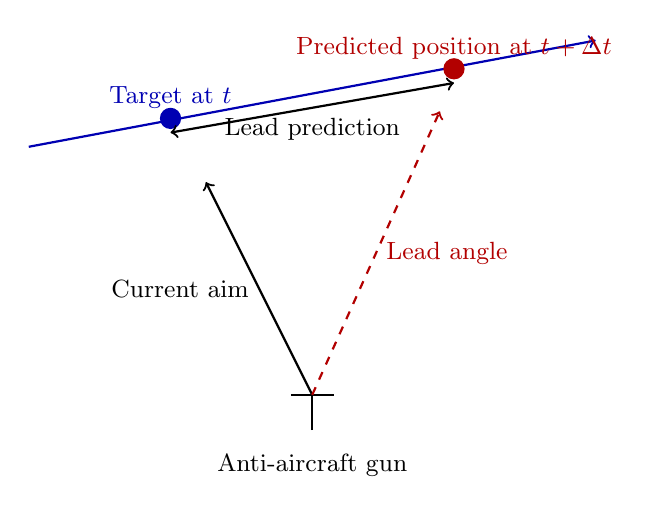
\begin{tikzpicture}[scale=0.9]
    % Aircraft trajectory
    \draw[thick, ->, blue!70!black] (0,4) -- (8,5.5);
    \fill[blue!70!black] (2,4.4) circle (0.15) node[above] {\small Target at $t$};
    \fill[red!70!black] (6,5.1) circle (0.15) node[above] {\small Predicted position at $t+\Delta t$};

    % Gun position
    \draw[thick] (4,0) -- (4,0.5);
    \draw[thick] (3.7,0.5) -- (4.3,0.5);
    \draw[thick, ->] (4,0.5) -- (2.5,3.5) node[midway, left] {\small Current aim};
    \draw[thick, ->, red!70!black, dashed] (4,0.5) -- (5.8,4.5) node[midway, right] {\small Lead angle};

    % Annotations
    \node at (4,-0.5) {\small Anti-aircraft gun};
    \draw[<->, thick] (2,4.2) -- (6,4.9) node[midway, below] {\small Lead prediction};
\end{tikzpicture}
\caption{The fire control problem: predicting target position requires derivative action, but noise amplification makes pure differentiation impractical.}
\label{fig:fire_control_problem}
\end{figure}

The mathematical problem was clear: to hit a moving target, the fire control system needed to \textit{predict} future position. In control terms, this meant incorporating derivative action---the system needed to respond not just to where the target \textit{was}, but to where it was \textit{going}. A simple proportional controller pointing the gun at the current target position would always lag behind.

\subsection{The Limitation of Pure PID Control}

Engineers quickly discovered that while PID control could theoretically provide the necessary derivative action, practical implementation faced severe obstacles. First, pure derivative action ($D(s) = K_d s$) amplifies high-frequency noise unboundedly, and radar tracking data corrupted by electrical noise and atmospheric effects produced unacceptable jitter in the control signal. Second, many servo systems had inadequate phase margin at the desired crossover frequency, meaning that simply increasing gain to improve tracking speed would push the system toward instability. Third, achieving both small steady-state error (requiring high loop gain) and fast, well-damped transient response (requiring adequate phase margin) seemed mutually exclusive with simple gain adjustment.

\subsection{Bode's Revolutionary Contribution}

Henrik Wade Bode, working at Bell Telephone Laboratories in the late 1930s and early 1940s, provided the theoretical framework that would resolve these dilemmas. His seminal work, ``Network Analysis and Feedback Amplifier Design'' (1945), introduced what we now call Bode plots and established the relationship between gain and phase in minimum-phase systems.

\begin{quotation}
\textit{``The advantage of logarithmic plots is that they reduce the problem of network synthesis to one of geometrical construction.''} --- H.W. Bode, 1945
\end{quotation}

Bode's key insight was that in the frequency domain, one could \textit{shape} the loop transfer function to achieve specific performance objectives. Rather than accepting whatever phase margin resulted from a given plant and controller combination, the engineer could design compensation networks that added phase precisely where needed.

\subsection{Lead Compensation: Filtered Derivative Action}

The lead compensator emerged as an elegant solution to the noise-amplification problem of pure derivative control. Consider the transfer function:

\begin{equation}
C(s) = K_c \frac{s + z}{s + p}, \quad \text{where } p > z
\label{eq:lead_compensator_intro}
\end{equation}

At low frequencies, this compensator behaves like a proportional gain of $K_c \cdot z/p$. At high frequencies, it approaches $K_c$---a constant gain rather than the unbounded amplification of a pure derivative. But crucially, in the mid-frequency range, the compensator provides \textit{phase lead}---it makes the output lead the input in phase, much like a derivative would.

\begin{figure}[htbp]
\centering
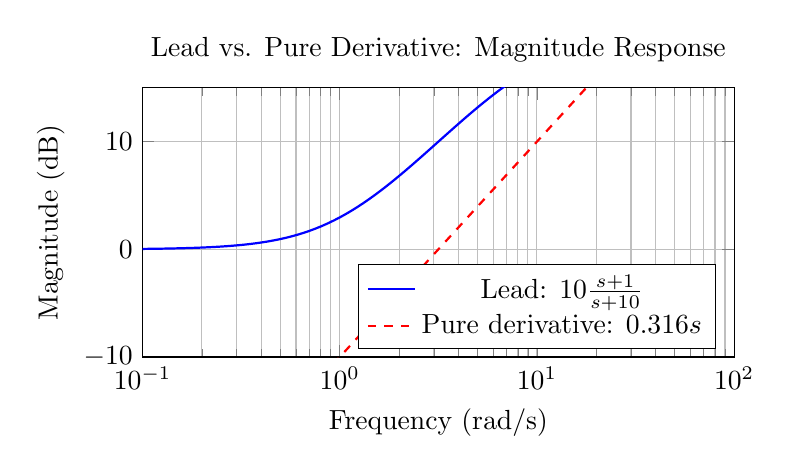
\begin{tikzpicture}
    \begin{semilogxaxis}[
        width=0.75\textwidth,
        height=5cm,
        xlabel={Frequency (rad/s)},
        ylabel={Magnitude (dB)},
        xmin=0.1, xmax=100,
        ymin=-10, ymax=15,
        grid=both,
        legend pos=south east,
        title={Lead vs. Pure Derivative: Magnitude Response}
    ]
    % Lead compensator: (s+1)/(s+10), Kc=10
    \addplot[thick, blue, domain=0.1:100, samples=100]
        {20*log10(10) + 10*log10(1+x^2) - 10*log10(100+x^2)};
    \addlegendentry{Lead: $10\frac{s+1}{s+10}$}

    % Pure derivative (scaled for comparison)
    \addplot[thick, red, dashed, domain=0.1:100, samples=100]
        {20*log10(x) - 10};
    \addlegendentry{Pure derivative: $0.316s$}
    \end{semilogxaxis}
\end{tikzpicture}
\caption{The lead compensator provides derivative-like behavior in the mid-frequency range while limiting high-frequency gain.}
\label{fig:lead_vs_derivative}
\end{figure}

The military significance was immediate: fire control systems could now incorporate predictive (derivative) action without being overwhelmed by radar noise. The M9 gun director, developed by Bell Labs and deployed in 1943, used analog lead-lag networks to achieve tracking accuracy that was considered miraculous at the time.

\subsection{Lag Compensation: Stable Integral Action}

The companion technique, lag compensation, addressed the steady-state accuracy problem. While integral control ($I(s) = K_i/s$) theoretically provides infinite DC gain, it also introduces 90 degrees of phase lag at all frequencies---often destabilizing the system.

The lag compensator:
\begin{equation}
C(s) = K_c \frac{s + z}{s + p}, \quad \text{where } z > p
\label{eq:lag_compensator_intro}
\end{equation}

provides \textit{high gain at low frequencies} (improving steady-state accuracy) while keeping the phase contribution near the crossover frequency small. The key design insight is to place the lag compensator's break frequencies well below the crossover frequency, so the system ``sees'' only the gain boost, not the phase penalty.

\subsection{Lead-Lag: The Best of Both Worlds}

By cascading lead and lag compensators, engineers could simultaneously increase phase margin at the crossover frequency through lead compensation, boost low-frequency gain for steady-state accuracy through lag compensation, and maintain bounded high-frequency gain for noise rejection.

This cascade approach became the standard methodology for precision servo design and remains widely used today.

%% ============================================================================
%% SECTION 2: MODERN APPLICATIONS
%% ============================================================================
\section{Modern Applications}
\label{sec:lead_lag_applications}

While born from military necessity, lead-lag compensation techniques have become ubiquitous across modern engineering. The following applications illustrate the continuing relevance of these classical methods.

\subsection{Hard Disk Drive Servo Systems}

Modern hard disk drives position read/write heads with nanometer precision over spinning platters at 7200 RPM or higher. The servo system must achieve settling times under 5 milliseconds for track-to-track seeks, maintain position accuracy within approximately 10 nanometers during read/write operations, and reject disturbances from disk flutter, bearing vibration, and external shocks.

Lead compensation provides the phase margin necessary for fast seeking, while lag compensation ensures the head remains precisely on track despite low-frequency disturbances. The constraints are severe: sampling rates exceed 20 kHz, and stability margins must account for manufacturing variations across millions of units.

\subsection{Antenna Tracking Systems}

Satellite communication and radio telescope systems require tracking moving objects (satellites in orbit, celestial sources) with arc-second precision. The challenges include large mechanical inertia of antenna structures, wind loading as a time-varying disturbance, and structural resonances that limit achievable bandwidth.

Lead-lag compensation shapes the loop response to maximize tracking bandwidth while providing robustness to resonance excitation. The Deep Space Network antennas, for example, use sophisticated lead-lag networks to maintain communication with spacecraft billions of kilometers away.

\subsection{Power System Stabilizers}

Synchronous generators in electric power grids can experience low-frequency oscillations (typically 0.2--2 Hz) that threaten system stability. Power system stabilizers (PSS) inject supplementary control signals into the generator's excitation system to damp these oscillations.

The PSS typically consists of cascaded lead-lag stages that provide phase compensation at the oscillation frequency. The design challenge is achieving sufficient phase lead without excessive high-frequency gain that could excite torsional resonances in the turbine-generator shaft.

\subsection{Precision Motion Control}

Industrial robots, CNC machines, and semiconductor manufacturing equipment all rely on lead-lag compensation for precise trajectory tracking. In photolithography systems, for example, the wafer stage must position a silicon wafer with errors below 1 nanometer while following complex scan patterns at speeds exceeding 1 meter per second.

%% ============================================================================
%% SECTION 3: MATHEMATICAL FOUNDATION
%% ============================================================================
\section{Mathematical Foundation}
\label{sec:lead_lag_math}

\subsection{The General First-Order Compensator}

Both lead and lag compensators share the same mathematical form:
\begin{equation}
\boxed{C(s) = K_c \frac{s + z}{s + p} = K_c \frac{\tau s + 1}{\alpha \tau s + 1}}
\label{eq:general_compensator}
\end{equation}

where $z = 1/\tau$ is the zero location, $p = 1/(\alpha\tau)$ is the pole location, and $\alpha = z/p = p_{\text{freq}}/z_{\text{freq}}$ in terms of break frequencies.

The distinction between lead and lag compensation lies solely in the relationship between $z$ and $p$. For a lead compensator, $p > z$ (equivalently, $\alpha > 1$), while for a lag compensator, $z > p$ (equivalently, $\alpha < 1$).

\subsection{Lead Compensator Analysis}

\subsubsection{Transfer Function and Bode Plot}

For the lead compensator with $p > z$, consider the standard form:
\begin{equation}
C_{\text{lead}}(s) = K_c \frac{s + z}{s + p} = K_c \cdot \frac{z}{p} \cdot \frac{s/z + 1}{s/p + 1}
\label{eq:lead_standard}
\end{equation}

The DC gain is $K_c \cdot z/p = K_c/\alpha < K_c$, while the high-frequency gain approaches $K_c$.

\begin{figure}[htbp]
\centering
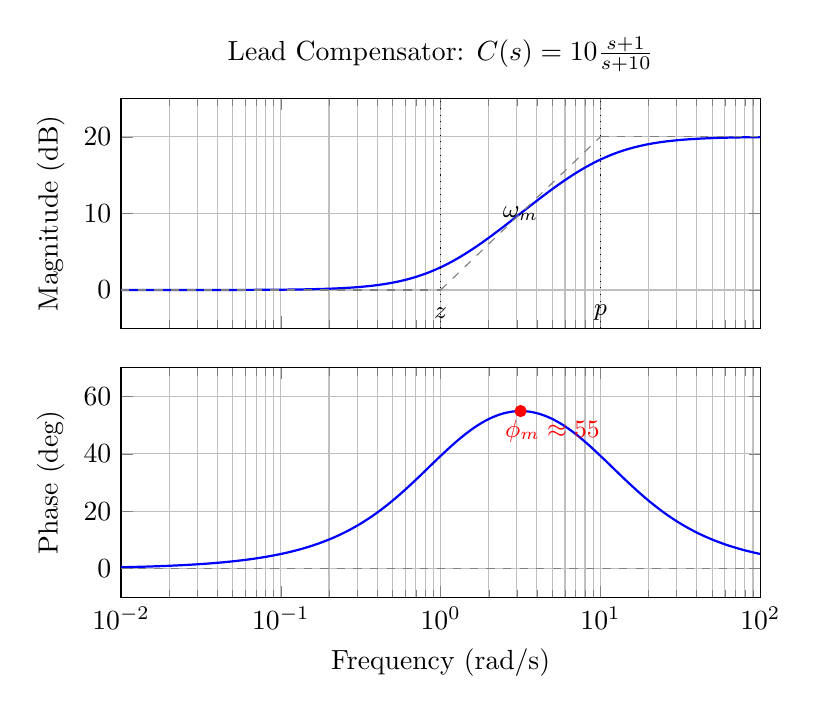
\begin{tikzpicture}
    % Magnitude plot
    \begin{semilogxaxis}[
        name=mag,
        width=0.8\textwidth,
        height=4.5cm,
        xlabel={},
        ylabel={Magnitude (dB)},
        xmin=0.01, xmax=100,
        ymin=-5, ymax=25,
        grid=both,
        xticklabels={},
        title={Lead Compensator: $C(s) = 10\frac{s+1}{s+10}$}
    ]
    % Lead compensator magnitude
    \addplot[thick, blue, domain=0.01:100, samples=200]
        {20*log10(10) + 10*log10(1+x^2) - 10*log10(100+x^2)};

    % Asymptotes
    \addplot[dashed, gray, domain=0.01:1] {20*log10(10) - 20};
    \addplot[dashed, gray, domain=1:10] {20*log10(10) - 20 + 20*log10(x)};
    \addplot[dashed, gray, domain=10:100] {20*log10(10)};

    % Mark frequencies
    \draw[dotted] (axis cs:1,-5) -- (axis cs:1,25);
    \draw[dotted] (axis cs:10,-5) -- (axis cs:10,25);
    \node at (axis cs:1,-3) {\small $z$};
    \node at (axis cs:10,-3) {\small $p$};
    \node at (axis cs:3.16,10) {\small $\omega_m$};
    \end{semilogxaxis}

    % Phase plot
    \begin{semilogxaxis}[
        at={(mag.south west)},
        anchor=north west,
        yshift=-0.5cm,
        width=0.8\textwidth,
        height=4.5cm,
        xlabel={Frequency (rad/s)},
        ylabel={Phase (deg)},
        xmin=0.01, xmax=100,
        ymin=-10, ymax=70,
        grid=both
    ]
    % Lead compensator phase
    \addplot[thick, blue, domain=0.01:100, samples=200]
        {atan(x) - atan(x/10)};

    % Mark maximum phase
    \addplot[only marks, mark=*, red] coordinates {(3.162, 54.9)};
    \node[red] at (axis cs:5,48) {\small $\phi_m \approx 55°$};

    % Asymptotes
    \draw[dashed, gray] (axis cs:0.01,0) -- (axis cs:100,0);
    \end{semilogxaxis}
\end{tikzpicture}
\caption{Bode plot of a lead compensator with $z=1$, $p=10$, $K_c=10$ (so $\alpha=10$). Maximum phase lead of approximately $55°$ occurs at $\omega_m = \sqrt{10} \approx 3.16$ rad/s.}
\label{fig:lead_bode}
\end{figure}

\subsubsection{Maximum Phase Lead}

The phase contribution of the lead compensator is:
\begin{equation}
\phi(\omega) = \tan^{-1}\left(\frac{\omega}{z}\right) - \tan^{-1}\left(\frac{\omega}{p}\right)
\label{eq:lead_phase}
\end{equation}

To find the frequency of maximum phase, we differentiate and set equal to zero:
\begin{align}
\frac{d\phi}{d\omega} &= \frac{z}{z^2 + \omega^2} - \frac{p}{p^2 + \omega^2} = 0
\end{align}

Solving for $\omega_m$:
\begin{equation}
\boxed{\omega_m = \sqrt{zp} = \frac{1}{\tau\sqrt{\alpha}}}
\label{eq:omega_max}
\end{equation}

The frequency of maximum phase is the \textit{geometric mean} of the zero and pole frequencies.

Substituting $\omega_m$ into the phase equation:
\begin{align}
\phi_m &= \tan^{-1}\left(\frac{\sqrt{zp}}{z}\right) - \tan^{-1}\left(\frac{\sqrt{zp}}{p}\right) \\
&= \tan^{-1}\left(\sqrt{\frac{p}{z}}\right) - \tan^{-1}\left(\sqrt{\frac{z}{p}}\right) \\
&= \tan^{-1}(\sqrt{\alpha}) - \tan^{-1}\left(\frac{1}{\sqrt{\alpha}}\right)
\end{align}

Using the identity $\tan^{-1}(x) - \tan^{-1}(1/x) = 2\tan^{-1}(x) - 90°$ for $x > 0$, or more directly via the sine function:

\begin{equation}
\boxed{\sin(\phi_m) = \frac{\alpha - 1}{\alpha + 1} = \frac{p - z}{p + z}}
\label{eq:phi_max}
\end{equation}

Equivalently:
\begin{equation}
\phi_m = \sin^{-1}\left(\frac{\alpha - 1}{\alpha + 1}\right)
\label{eq:phi_max_explicit}
\end{equation}

\begin{table}[htbp]
\centering
\caption{Maximum Phase Lead vs. $\alpha = p/z$}
\label{tab:alpha_phase}
\begin{tabular}{ccc}
\toprule
$\alpha$ & $\sin(\phi_m)$ & $\phi_m$ (degrees) \\
\midrule
2 & 0.333 & 19.5 \\
3 & 0.500 & 30.0 \\
4 & 0.600 & 36.9 \\
5 & 0.667 & 41.8 \\
10 & 0.818 & 54.9 \\
20 & 0.905 & 64.8 \\
\bottomrule
\end{tabular}
\end{table}

\textbf{Design insight:} Single-stage lead compensators are typically limited to providing about $55°$--$60°$ of phase lead. For larger phase margins, multiple cascaded stages or a lead-lag design should be considered.

\subsubsection{Gain at Maximum Phase Frequency}

At $\omega = \omega_m = \sqrt{zp}$, the magnitude of the compensator is:
\begin{align}
|C(j\omega_m)| &= K_c \frac{|j\omega_m + z|}{|j\omega_m + p|} = K_c \sqrt{\frac{\omega_m^2 + z^2}{\omega_m^2 + p^2}} \\
&= K_c \sqrt{\frac{zp + z^2}{zp + p^2}} = K_c \sqrt{\frac{z(p+z)}{p(p+z)}} = K_c \sqrt{\frac{z}{p}}
\end{align}

In decibels:
\begin{equation}
|C(j\omega_m)|_{\text{dB}} = 20\log_{10}(K_c) + 10\log_{10}\left(\frac{z}{p}\right) = 20\log_{10}(K_c) - 10\log_{10}(\alpha)
\label{eq:gain_at_omega_m}
\end{equation}

This is exactly halfway (in dB) between the low-frequency and high-frequency asymptotes.

\subsubsection{Lead Compensator Design Procedure}

Given specifications for phase margin improvement $\phi_{\text{needed}}$ and desired crossover frequency $\omega_c$, the design proceeds as follows. First, determine the required $\alpha$ by adding 5°--12° safety margin to $\phi_{\text{needed}}$ to account for the gain increase at $\omega_m$, then solve:
\begin{equation}
\alpha = \frac{1 + \sin(\phi_m)}{1 - \sin(\phi_m)}
\label{eq:alpha_from_phi}
\end{equation}
Second, calculate the zero and pole locations by placing $\omega_m = \omega_c$ (desired crossover frequency):
\begin{align}
z &= \frac{\omega_c}{\sqrt{\alpha}} \\
p &= \omega_c \sqrt{\alpha}
\label{eq:zp_from_omega}
\end{align}
Third, determine $K_c$ by adjusting it so the compensated loop gain magnitude equals 0 dB at $\omega_c$. Since the lead compensator contributes $-10\log_{10}(\alpha)$ dB at $\omega_m$:
\begin{equation}
K_c = \sqrt{\alpha} \cdot |G(j\omega_c)|^{-1}
\label{eq:Kc_lead}
\end{equation}
where $G(s)$ is the uncompensated plant.

\subsection{Lag Compensator Analysis}

\subsubsection{Transfer Function and Bode Plot}

For the lag compensator with $z > p$, we write:
\begin{equation}
C_{\text{lag}}(s) = K_c \frac{s + z}{s + p} = K_c \cdot \frac{z}{p} \cdot \frac{s/z + 1}{s/p + 1}, \quad z > p
\label{eq:lag_standard}
\end{equation}

Now $\beta = z/p > 1$, and the DC gain is $K_c \cdot \beta > K_c$.

\begin{figure}[htbp]
\centering
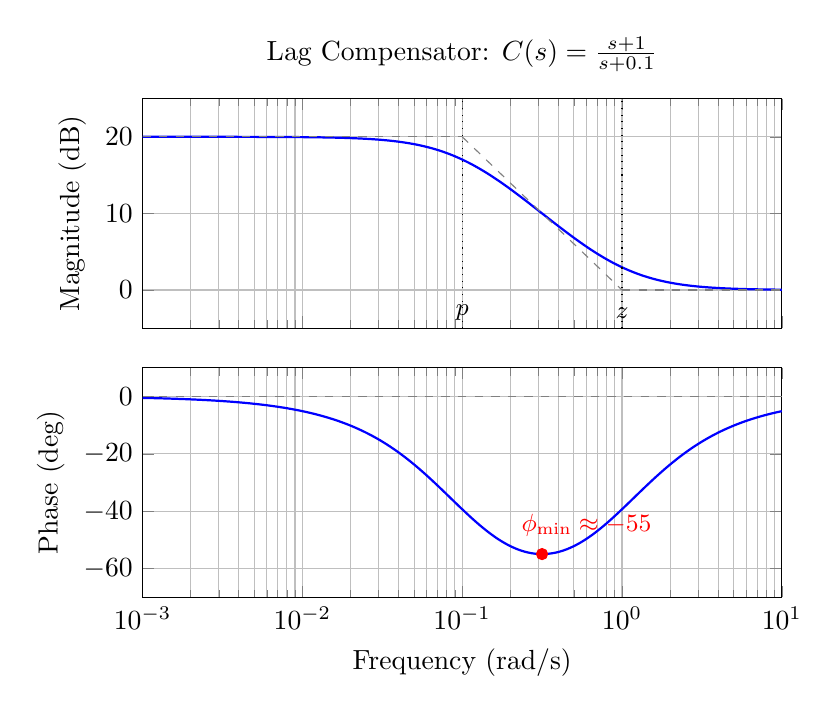
\begin{tikzpicture}
    % Magnitude plot
    \begin{semilogxaxis}[
        name=maglag,
        width=0.8\textwidth,
        height=4.5cm,
        xlabel={},
        ylabel={Magnitude (dB)},
        xmin=0.001, xmax=10,
        ymin=-5, ymax=25,
        grid=both,
        xticklabels={},
        title={Lag Compensator: $C(s) = \frac{s+1}{s+0.1}$}
    ]
    % Lag compensator magnitude
    \addplot[thick, blue, domain=0.001:10, samples=200]
        {10*log10(1+x^2) - 10*log10(0.01+x^2)};

    % Asymptotes
    \addplot[dashed, gray, domain=0.001:0.1] {20};
    \addplot[dashed, gray, domain=0.1:1] {20 - 20*log10(x/0.1)};
    \addplot[dashed, gray, domain=1:10] {0};

    % Mark frequencies
    \draw[dotted] (axis cs:0.1,-5) -- (axis cs:0.1,25);
    \draw[dotted] (axis cs:1,-5) -- (axis cs:1,25);
    \node at (axis cs:0.1,-3) {\small $p$};
    \node at (axis cs:1,-3) {\small $z$};
    \end{semilogxaxis}

    % Phase plot
    \begin{semilogxaxis}[
        at={(maglag.south west)},
        anchor=north west,
        yshift=-0.5cm,
        width=0.8\textwidth,
        height=4.5cm,
        xlabel={Frequency (rad/s)},
        ylabel={Phase (deg)},
        xmin=0.001, xmax=10,
        ymin=-70, ymax=10,
        grid=both
    ]
    % Lag compensator phase
    \addplot[thick, blue, domain=0.001:10, samples=200]
        {atan(x) - atan(x/0.1)};

    % Mark maximum phase lag
    \addplot[only marks, mark=*, red] coordinates {(0.316, -54.9)};
    \node[red] at (axis cs:0.6,-45) {\small $\phi_{\min} \approx -55°$};

    \draw[dashed, gray] (axis cs:0.001,0) -- (axis cs:10,0);
    \end{semilogxaxis}
\end{tikzpicture}
\caption{Bode plot of a lag compensator with $p=0.1$, $z=1$ (so $\beta=10$). The DC gain is boosted by 20 dB, but significant phase lag occurs in the transition region.}
\label{fig:lag_bode}
\end{figure}

\subsubsection{Design Philosophy}

The lag compensator provides two key benefits. First, the factor $\beta = z/p$ provides a low-frequency gain boost that increases the DC loop gain, thereby reducing steady-state error. Second, by placing both $z$ and $p$ well below the crossover frequency $\omega_c$, the phase lag contribution at $\omega_c$ remains small (typically 5°--10°), ensuring minimal phase impact at crossover.

\subsubsection{Lag Compensator Design Procedure}

Given the required steady-state error improvement and existing phase margin, the design procedure proceeds as follows. First, determine $\beta$ by calculating the ratio of current steady-state error to desired error: $\beta = e_{\text{ss,current}}/e_{\text{ss,desired}}$. Second, find the current crossover frequency $\omega_c$ from the uncompensated Bode plot. Third, place the lag compensator zero by choosing $z$ such that $z \leq \omega_c / 10$, which ensures the phase lag at $\omega_c$ is acceptably small:
\begin{equation}
\phi_{\text{lag}}(\omega_c) = \tan^{-1}\left(\frac{\omega_c}{z}\right) - \tan^{-1}\left(\frac{\omega_c}{p}\right) \approx -5° \text{ to } -10°
\end{equation}
Fourth, calculate the pole location as $p = z/\beta$. Fifth, set $K_c$, which is typically equal to 1 since the gain boost comes from the $\beta$ factor; adjust if needed to maintain the original crossover frequency.

\subsection{Lead-Lag Compensator}

When both increased phase margin and improved steady-state accuracy are required, a lead-lag compensator cascades both elements:

\begin{equation}
\boxed{C_{\text{lead-lag}}(s) = K_c \underbrace{\frac{s + z_{\text{lead}}}{s + p_{\text{lead}}}}_{\text{Lead stage}} \cdot \underbrace{\frac{s + z_{\text{lag}}}{s + p_{\text{lag}}}}_{\text{Lag stage}}}
\label{eq:lead_lag}
\end{equation}

where $p_{\text{lead}} > z_{\text{lead}}$ and $z_{\text{lag}} > p_{\text{lag}}$.

\begin{figure}[htbp]
\centering
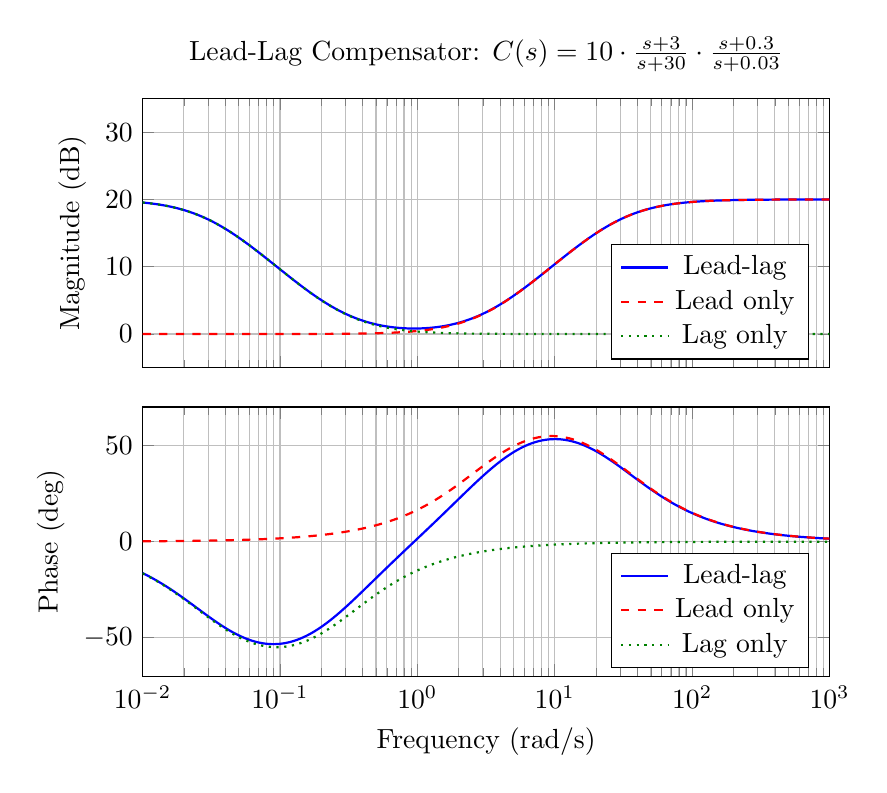
\begin{tikzpicture}
    % Magnitude plot
    \begin{semilogxaxis}[
        name=magleadlag,
        width=0.85\textwidth,
        height=5cm,
        xlabel={},
        ylabel={Magnitude (dB)},
        xmin=0.01, xmax=1000,
        ymin=-5, ymax=35,
        grid=both,
        xticklabels={},
        title={Lead-Lag Compensator: $C(s) = 10 \cdot \frac{s+3}{s+30} \cdot \frac{s+0.3}{s+0.03}$},
        legend pos=south east
    ]
    % Lead-lag compensator magnitude
    \addplot[thick, blue, domain=0.01:1000, samples=300]
        {20*log10(10) + 10*log10(9+x^2) - 10*log10(900+x^2) + 10*log10(0.09+x^2) - 10*log10(0.0009+x^2)};
    \addlegendentry{Lead-lag}

    % Lead only
    \addplot[thick, red, dashed, domain=0.01:1000, samples=300]
        {20*log10(10) + 10*log10(9+x^2) - 10*log10(900+x^2)};
    \addlegendentry{Lead only}

    % Lag only
    \addplot[thick, green!50!black, dotted, domain=0.01:1000, samples=300]
        {10*log10(0.09+x^2) - 10*log10(0.0009+x^2)};
    \addlegendentry{Lag only}
    \end{semilogxaxis}

    % Phase plot
    \begin{semilogxaxis}[
        at={(magleadlag.south west)},
        anchor=north west,
        yshift=-0.5cm,
        width=0.85\textwidth,
        height=5cm,
        xlabel={Frequency (rad/s)},
        ylabel={Phase (deg)},
        xmin=0.01, xmax=1000,
        ymin=-70, ymax=70,
        grid=both,
        legend pos=south east
    ]
    % Lead-lag phase
    \addplot[thick, blue, domain=0.01:1000, samples=300]
        {atan(x/3) - atan(x/30) + atan(x/0.3) - atan(x/0.03)};
    \addlegendentry{Lead-lag}

    % Lead only phase
    \addplot[thick, red, dashed, domain=0.01:1000, samples=300]
        {atan(x/3) - atan(x/30)};
    \addlegendentry{Lead only}

    % Lag only phase
    \addplot[thick, green!50!black, dotted, domain=0.01:1000, samples=300]
        {atan(x/0.3) - atan(x/0.03)};
    \addlegendentry{Lag only}
    \end{semilogxaxis}
\end{tikzpicture}
\caption{Bode plot of a lead-lag compensator showing individual contributions. The lag stage boosts low-frequency gain by 20 dB while the lead stage provides phase lead near the crossover frequency.}
\label{fig:lead_lag_bode}
\end{figure}

\subsubsection{Design Approach}

The design approach for lead-lag compensation proceeds in three stages. First, design the lead stage by determining the phase margin improvement needed and placing the lead compensator to provide maximum phase at the desired crossover frequency. Second, design the lag stage by calculating the additional low-frequency gain needed for steady-state accuracy and placing the lag zero at least one decade below the crossover frequency. Third, verify stability by checking that the total phase margin with both stages is adequate, accounting for the small phase lag contribution from the lag stage at crossover.

\subsection{Root Locus Interpretation}

Lead-lag compensation can also be understood through root locus analysis.

\begin{figure}[htbp]
\centering
\begin{tikzpicture}[scale=1.1]
    % Axes
    \draw[->] (-5,0) -- (1,0) node[right] {Re};
    \draw[->] (0,-3) -- (0,3) node[above] {Im};

    % Original poles (plant)
    \node[red, cross out, draw, thick] at (-1,0) {};
    \node[red, cross out, draw, thick] at (-2,1.5) {};
    \node[red, cross out, draw, thick] at (-2,-1.5) {};
    \node[red, below] at (-1,-0.3) {\small Plant poles};

    % Lead compensator zero
    \node[blue, circle, draw, thick, inner sep=2pt] at (-3,0) {};
    \node[blue, below] at (-3,-0.3) {\small Lead zero};

    % Lead compensator pole
    \node[blue, cross out, draw, thick] at (-4.5,0) {};
    \node[blue, below] at (-4.5,-0.3) {\small Lead pole};

    % Root locus branches (sketched)
    \draw[thick, purple, ->] (-1,0) .. controls (-1.5,0.3) and (-2,0.5) .. (-2.5,0.3);
    \draw[thick, purple, ->] (-2,1.5) .. controls (-2.3,1.2) and (-2.6,0.8) .. (-2.8,0.4);
    \draw[thick, purple, ->] (-2,-1.5) .. controls (-2.3,-1.2) and (-2.6,-0.8) .. (-2.8,-0.4);

    % Desired pole region
    \draw[dashed, gray] (-4,2.5) -- (-1.5,0) -- (-4,-2.5);
    \node[gray] at (-3.5,2) {\small Desired region};

    % Legend
    \node[right] at (0.5,2.5) {\small $\times$ Poles};
    \node[right] at (0.5,2) {\small $\circ$ Zeros};
\end{tikzpicture}
\caption{Effect of lead compensator on root locus. The compensator zero ``pulls'' the locus toward the left half-plane, while the far-left pole has minimal effect on dominant dynamics.}
\label{fig:lead_root_locus}
\end{figure}

\textbf{Lead compensator effect:} The zero attracts root locus branches, pulling closed-loop poles toward the left half-plane (faster response, better damping). The pole is placed far left so its branch quickly leaves the region of dominant dynamics.

\textbf{Lag compensator effect:} Both the zero and pole are near the origin. The pole-zero pair (nearly canceling) minimally affects the root locus shape but allows higher loop gain $K$ before instability, improving steady-state accuracy.

%% ============================================================================
%% SECTION 4: PRACTICAL EXPERIMENT
%% ============================================================================
\section{Practical Experiment: Motor Position Control with Lead Compensation}
\label{sec:lead_lag_experiment}

\subsection{Objective}

This experiment demonstrates the practical benefits of lead compensation by implementing a position servo on a DC motor. You will characterize the uncompensated system response, design a lead compensator to improve phase margin, implement the compensator digitally on an Arduino, and measure and compare step responses before and after compensation.

\subsection{Required Equipment}

\begin{table}[htbp]
\centering
\caption{Equipment Required for Lead Compensation Experiment}
\begin{tabular}{ll}
\toprule
\textbf{Component} & \textbf{Specification} \\
\midrule
DC motor with encoder & 12V geared motor, 48 CPR encoder \\
Microcontroller & Arduino Mega or similar \\
Motor driver & L298N or equivalent H-bridge \\
Potentiometer & 10k$\Omega$ for setpoint input \\
Power supply & 12V DC \\
Visualization & Oscilloscope or serial plotter \\
Software & Computer with Arduino IDE \\
\bottomrule
\end{tabular}
\end{table}

\subsection{System Model}

A DC motor position system can be approximated as:
\begin{equation}
G(s) = \frac{\theta(s)}{V(s)} = \frac{K_m}{s(\tau_m s + 1)}
\label{eq:motor_plant}
\end{equation}

where $K_m$ is the motor gain constant and $\tau_m$ is the mechanical time constant. With proportional control $K_p$, the open-loop transfer function is:
\begin{equation}
L(s) = \frac{K_p K_m}{s(\tau_m s + 1)}
\label{eq:motor_loop}
\end{equation}

This system has 90° of phase lag from the integrator and additional lag from the motor pole, making the phase margin sensitive to gain selection.

\subsection{Experiment Procedure}

\subsubsection{Step 1: System Identification}

First, characterize your motor's parameters:

\begin{algorithm}
\caption{Motor Identification via Step Response Test}
\begin{algorithmic}[1]
\State \textbf{Initialize:}
\State \hspace{1em} Configure motor PWM and direction pins as outputs
\State \hspace{1em} Configure encoder channels A and B as inputs with pull-up resistors
\State \hspace{1em} Attach interrupt to encoder channel A on rising edge
\State \hspace{1em} Set $\text{encoderCount} \gets 0$
\State
\State \textbf{Apply Step Input:}
\State \hspace{1em} Set motor direction to forward
\State \hspace{1em} Set PWM duty cycle to 50\%
\State \hspace{1em} Record $\text{startTime} \gets \text{currentTime}$
\State
\State \textbf{Data Logging Loop:}
\While{$\text{currentTime} - \text{startTime} < 2000$ ms}
    \State Output timestamp and encoder count to serial port
    \State Wait 10 ms
\EndWhile
\State Set PWM duty cycle to 0\% (stop motor)
\State
\State \textbf{Encoder Interrupt Service Routine:}
\If{encoder channel B is LOW}
    \State $\text{encoderCount} \gets \text{encoderCount} + 1$
\Else
    \State $\text{encoderCount} \gets \text{encoderCount} - 1$
\EndIf
\end{algorithmic}
\end{algorithm}

From the velocity response data, identify $K_m$ (steady-state velocity per volt) and $\tau_m$ (time to reach 63\% of final velocity).

\subsubsection{Step 2: Proportional Control Baseline}

Implement proportional control and observe the step response:

\begin{algorithm}
\caption{Proportional Position Control Baseline}
\begin{algorithmic}[1]
\State \textbf{Parameters:} $K_p \gets 5.0$ (proportional gain, start low)
\State
\Loop
    \State Read setpoint from potentiometer (analog input)
    \State Map raw value to range $[-500, 500]$ counts
    \State $\text{error} \gets \text{setpoint} - \text{encoderCount}$
    \State $\text{controlSignal} \gets K_p \cdot \text{error}$
    \State Saturate controlSignal to range $[-255, 255]$
    \State
    \If{$\text{controlSignal} \geq 0$}
        \State Set motor direction to forward
        \State Set PWM to controlSignal
    \Else
        \State Set motor direction to reverse
        \State Set PWM to $|\text{controlSignal}|$
    \EndIf
    \State
    \State Log timestamp, setpoint, and encoder count
    \State Wait 5 ms (200 Hz sample rate)
\EndLoop
\end{algorithmic}
\end{algorithm}

Increase $K_p$ until the system shows significant overshoot (indicating low phase margin). Record this gain and the step response characteristics.

\subsubsection{Step 3: Lead Compensator Design}

For a typical motor with $\tau_m = 0.05$ s and desired crossover at $\omega_c = 30$ rad/s:

\textbf{Design calculations:} The desired phase margin is 50°, which means we need $\phi_m \approx 55°$ when accounting for gain change. From $\sin(55°) = 0.819 = (\alpha-1)/(\alpha+1)$, we obtain $\alpha = 10$. The zero location is then $z = \omega_c/\sqrt{\alpha} = 30/\sqrt{10} \approx 9.5$ rad/s, and the pole location is $p = \omega_c \sqrt{\alpha} = 30\sqrt{10} \approx 95$ rad/s.

In the discrete domain (Tustin transform with $T_s = 0.005$ s):
\begin{equation}
C(z) = K_c \frac{1 + a_1 z^{-1}}{1 + b_1 z^{-1}}
\end{equation}

\subsubsection{Step 4: Digital Lead Compensator Implementation}

\begin{algorithm}
\caption{Digital Lead Compensator Implementation}
\begin{algorithmic}[1]
\State \textbf{Parameters:}
\State \hspace{1em} $K_p \gets 8.0$ (higher gain now stable with compensation)
\State \hspace{1em} $a_1 \gets -0.907$ (Tustin coefficient for zero)
\State \hspace{1em} $b_1 \gets -0.621$ (Tustin coefficient for pole)
\State \hspace{1em} $K_c \gets 3.16$ ($\sqrt{\alpha}$ compensation factor)
\State \hspace{1em} $T_s \gets 5$ ms (sample period)
\State
\State \textbf{State Variables:}
\State \hspace{1em} $x_{\text{prev}} \gets 0$, $y_{\text{prev}} \gets 0$
\State
\Function{LeadCompensator}{$x$}
    \State $y \gets -b_1 \cdot y_{\text{prev}} + K_c \cdot (x + a_1 \cdot x_{\text{prev}})$
    \State $x_{\text{prev}} \gets x$
    \State $y_{\text{prev}} \gets y$
    \State \Return $y$
\EndFunction
\State
\State \textbf{Main Control Loop:}
\Loop
    \If{$T_s$ has elapsed since last sample}
        \State Read setpoint from potentiometer
        \State Map to range $[-500, 500]$ counts
        \State $\text{error} \gets \text{setpoint} - \text{encoderCount}$
        \State $\text{propOutput} \gets K_p \cdot \text{error}$
        \State $\text{compOutput} \gets \text{LeadCompensator}(\text{propOutput})$
        \State Saturate compOutput to $[-255, 255]$
        \State Apply compOutput to motor (set direction and PWM)
        \State Log timestamp, setpoint, and encoder count
    \EndIf
\EndLoop
\end{algorithmic}
\end{algorithm}

\subsection{Expected Results}

\begin{figure}[htbp]
\centering
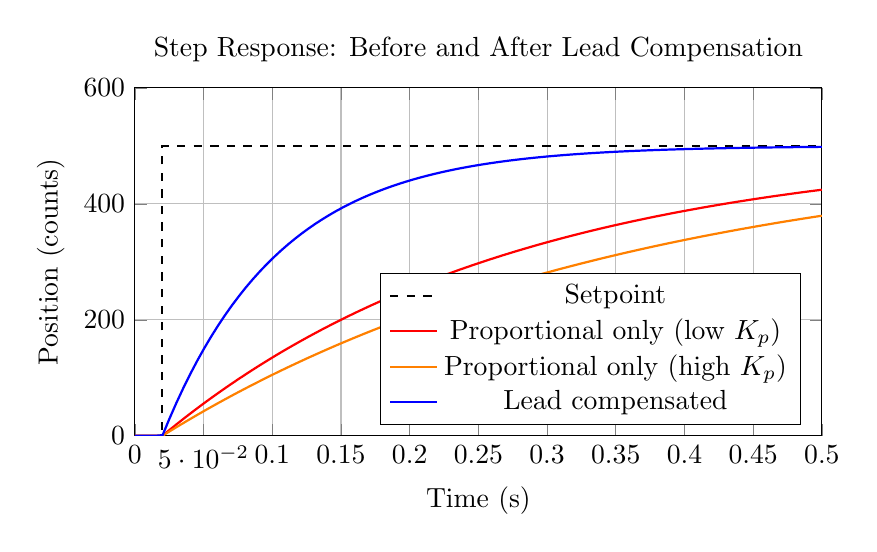
\begin{tikzpicture}
    \begin{axis}[
        width=0.85\textwidth,
        height=6cm,
        xlabel={Time (s)},
        ylabel={Position (counts)},
        xmin=0, xmax=0.5,
        ymin=0, ymax=600,
        grid=both,
        legend pos=south east,
        title={Step Response: Before and After Lead Compensation}
    ]
    % Setpoint
    \addplot[thick, black, dashed] coordinates {(0,0) (0.02,0) (0.02,500) (0.5,500)};
    \addlegendentry{Setpoint}

    % Uncompensated (low Kp, slow)
    \addplot[thick, red, domain=0:0.5, samples=100]
        {500*(1 - exp(-4*max(x-0.02,0))*(cos(6*max(x-0.02,0)) + 0.67*sin(6*max(x-0.02,0))))*(x>0.02)};
    \addlegendentry{Proportional only (low $K_p$)}

    % Uncompensated (high Kp, oscillatory)
    \addplot[thick, orange, domain=0:0.5, samples=100]
        {500*(1 - exp(-3*max(x-0.02,0))*(cos(15*max(x-0.02,0)) + 0.2*sin(15*max(x-0.02,0))))*(x>0.02)};
    \addlegendentry{Proportional only (high $K_p$)}

    % Lead compensated
    \addplot[thick, blue, domain=0:0.5, samples=100]
        {500*(1 - exp(-12*max(x-0.02,0))*(cos(8*max(x-0.02,0)) + 1.5*sin(8*max(x-0.02,0))))*(x>0.02)};
    \addlegendentry{Lead compensated}
    \end{axis}
\end{tikzpicture}
\caption{Comparison of step responses. The lead compensator enables faster response with less overshoot compared to high-gain proportional control alone.}
\label{fig:step_response_comparison}
\end{figure}

You should observe the following behavior. With proportional control only, the system exhibits either slow response when using low $K_p$ or significant overshoot and oscillation when using high $K_p$. With lead compensation, however, the system achieves faster rise time \textit{and} reduced overshoot simultaneously. The phase margin improvement allows higher effective gain without sacrificing stability.

\subsection{Verifying Phase Margin Improvement}

While direct frequency response measurement requires specialized equipment, you can estimate phase margin from the step response:

\begin{equation}
\text{Overshoot} \approx e^{-\pi\zeta/\sqrt{1-\zeta^2}} \implies \zeta \implies \text{PM} \approx 100\zeta \text{ (degrees, rough estimate)}
\end{equation}

Compare the overshoot before and after compensation to verify improved damping.

%% ============================================================================
%% SECTION 5: EXAMPLE PROBLEMS
%% ============================================================================
\section{Example Problems}
\label{sec:lead_lag_examples}

\begin{examplebox}[Example 14.1: Lead Compensator for Specified Phase Margin]
\textbf{Problem:} A unity-feedback system has plant transfer function:
\[
G(s) = \frac{10}{s(s+2)}
\]
Design a lead compensator to achieve a phase margin of 45° at a crossover frequency of 4 rad/s.

\textbf{Solution:}

\textit{Step 1: Analyze uncompensated system at desired crossover.}

At $\omega = 4$ rad/s:
\begin{align}
|G(j4)| &= \frac{10}{|j4| \cdot |j4+2|} = \frac{10}{4 \cdot \sqrt{16+4}} = \frac{10}{4 \cdot \sqrt{20}} = \frac{10}{17.89} = 0.559 \\
|G(j4)|_{\text{dB}} &= 20\log_{10}(0.559) = -5.05 \text{ dB}
\end{align}

\begin{align}
\angle G(j4) &= -90° - \tan^{-1}(4/2) = -90° - 63.4° = -153.4°
\end{align}

Uncompensated phase margin: $180° - 153.4° = 26.6°$.

\textit{Step 2: Determine required phase lead.}

Phase needed: $45° - 26.6° = 18.4°$.

Add 10° safety margin for gain change: $\phi_m = 28.4° \approx 30°$.

\textit{Step 3: Calculate $\alpha$.}

From $\sin(30°) = 0.5 = (\alpha-1)/(\alpha+1)$:
\[
0.5(\alpha+1) = \alpha - 1 \implies 0.5\alpha + 0.5 = \alpha - 1 \implies \alpha = 3
\]

\textit{Step 4: Calculate zero and pole.}

\begin{align}
z &= \frac{\omega_c}{\sqrt{\alpha}} = \frac{4}{\sqrt{3}} = 2.31 \text{ rad/s} \\
p &= \omega_c \sqrt{\alpha} = 4\sqrt{3} = 6.93 \text{ rad/s}
\end{align}

\textit{Step 5: Determine $K_c$.}

The compensator magnitude at $\omega_c$ is $1/\sqrt{\alpha} = 1/\sqrt{3} = 0.577$ (i.e., $-4.77$ dB).

Combined magnitude at $\omega_c$: $-5.05 - 4.77 + 20\log_{10}(K_c) = 0$ dB.

Solving: $20\log_{10}(K_c) = 9.82$, so $K_c = 3.10$.

\textbf{Final compensator:}
\[
\boxed{C(s) = 3.10 \cdot \frac{s + 2.31}{s + 6.93}}
\]

\textit{Verification:}

At $\omega = 4$:
\begin{align}
|C(j4)| &= 3.10 \cdot \frac{\sqrt{16 + 5.34}}{\sqrt{16 + 48.0}} = 3.10 \cdot \frac{4.62}{8.00} = 1.79 \\
|L(j4)| &= |C(j4)||G(j4)| = 1.79 \times 0.559 = 1.00 \quad \checkmark
\end{align}

\begin{align}
\angle C(j4) &= \tan^{-1}(4/2.31) - \tan^{-1}(4/6.93) = 60.0° - 30.0° = 30° \\
\angle L(j4) &= -153.4° + 30° = -123.4° \\
\text{PM} &= 180° - 123.4° = 56.6° > 45° \quad \checkmark
\end{align}

The achieved phase margin exceeds the specification, as expected due to our safety margin.
\end{examplebox}

\begin{examplebox}[Example 14.2: Lag Compensator for Steady-State Error]

\textbf{Problem:} A unity-feedback system has:
\[
G(s) = \frac{5}{s(s+1)(s+5)}
\]
The current phase margin is 35°, which is acceptable. Design a lag compensator to reduce the steady-state error to a ramp input by a factor of 10.

\textbf{Solution:}

\textit{Step 1: Determine current velocity error constant.}

\[
K_v = \lim_{s \to 0} s \cdot G(s) = \lim_{s \to 0} s \cdot \frac{5}{s(s+1)(s+5)} = \frac{5}{1 \cdot 5} = 1 \text{ s}^{-1}
\]

Current steady-state error to unit ramp: $e_{ss} = 1/K_v = 1$.

\textit{Step 2: Required improvement.}

To reduce error by factor of 10: need $K_v = 10$ s$^{-1}$.

Therefore $\beta = 10$.

\textit{Step 3: Find current crossover frequency.}

Setting $|G(j\omega_c)| = 1$:
\[
\frac{5}{\omega_c \sqrt{\omega_c^2 + 1} \sqrt{\omega_c^2 + 25}} = 1
\]

Solving numerically: $\omega_c \approx 1.26$ rad/s.

\textit{Step 4: Place lag compensator.}

Choose $z = \omega_c / 10 = 0.126$ rad/s.

Then $p = z/\beta = 0.126/10 = 0.0126$ rad/s.

\textbf{Final compensator:}
\[
\boxed{C(s) = \frac{s + 0.126}{s + 0.0126} = \frac{s + 0.126}{s + 0.0126}}
\]

\textit{Verification of phase impact:}

At $\omega_c = 1.26$ rad/s:
\begin{align}
\angle C(j\omega_c) &= \tan^{-1}(1.26/0.126) - \tan^{-1}(1.26/0.0126) \\
&= \tan^{-1}(10) - \tan^{-1}(100) \\
&= 84.3° - 89.4° = -5.1°
\end{align}

Phase margin reduction is only about 5°, leaving approximately 30° phase margin.

New velocity constant: $K_v = 10 \cdot 1 = 10$ s$^{-1}$ $\checkmark$
\end{examplebox}

\subsection{Example 14.3: Maximum Phase Lead Calculation}

\textbf{Problem:} A lead compensator has the form:
\[
C(s) = K \frac{s + 4}{s + 20}
\]
Find (a) the maximum phase lead, (b) the frequency at which it occurs, and (c) the compensator gain at that frequency in dB (assuming $K=1$).

\textbf{Solution:}

(a) \textit{Maximum phase lead:}

Here $z = 4$, $p = 20$, so $\alpha = p/z = 5$.

\[
\phi_m = \sin^{-1}\left(\frac{\alpha - 1}{\alpha + 1}\right) = \sin^{-1}\left(\frac{5-1}{5+1}\right) = \sin^{-1}(0.667) = \boxed{41.8°}
\]

(b) \textit{Frequency of maximum phase:}

\[
\omega_m = \sqrt{zp} = \sqrt{4 \times 20} = \sqrt{80} = \boxed{8.94 \text{ rad/s}}
\]

(c) \textit{Gain at $\omega_m$:}

\[
|C(j\omega_m)| = \sqrt{\frac{z}{p}} = \sqrt{\frac{4}{20}} = \sqrt{0.2} = 0.447
\]
\[
|C(j\omega_m)|_{\text{dB}} = 20\log_{10}(0.447) = \boxed{-7.0 \text{ dB}}
\]

Alternatively: $-10\log_{10}(\alpha) = -10\log_{10}(5) = -7.0$ dB.

\subsection{Example 14.4: Lead-Lag Design for Combined Specifications}

\textbf{Problem:} Design a lead-lag compensator for:
\[
G(s) = \frac{4}{s(s+2)}
\]
Specifications: (1) Phase margin $\geq 50°$, (2) Velocity error constant $K_v \geq 20$ s$^{-1}$.

\textbf{Solution:}

\textit{Step 1: Analyze uncompensated system.}

Current $K_v = \lim_{s \to 0} s \cdot \frac{4}{s(s+2)} = \frac{4}{2} = 2$ s$^{-1}$.

Need to increase $K_v$ by factor of 10, so $\beta = 10$ for lag stage.

Find crossover where uncompensated PM $\approx$ 50° (before adding lead):

At $\omega = 1$ rad/s: $\angle G = -90° - \tan^{-1}(0.5) = -116.6°$, PM = 63.4°.

At $\omega = 2$ rad/s: $\angle G = -90° - \tan^{-1}(1) = -135°$, PM = 45°.

Target $\omega_c \approx 1.5$ rad/s for 50° margin with lead assistance.

\textit{Step 2: Design lag compensator.}

Place lag zero at $\omega_c/10 = 0.15$ rad/s.

Lag pole at $p = 0.15/10 = 0.015$ rad/s.

\[
C_{\text{lag}}(s) = \frac{s + 0.15}{s + 0.015}
\]

This provides the $10\times$ gain boost at DC.

\textit{Step 3: Design lead compensator.}

After lag compensation, need to verify phase margin at new crossover and add lead if needed.

With $\beta = 10$ gain boost, the new crossover shifts higher. Recalculating:

For PM = 50° at $\omega_c = 3$ rad/s (approximate new crossover):

Phase needed from lead: approximately $20°$.

With $\phi_m = 25°$ (including margin): $\sin(25°) = 0.423 = (\alpha-1)/(\alpha+1)$, giving $\alpha = 2.47 \approx 2.5$.

\begin{align}
z_{\text{lead}} &= \frac{3}{\sqrt{2.5}} = 1.90 \text{ rad/s} \\
p_{\text{lead}} &= 3\sqrt{2.5} = 4.74 \text{ rad/s}
\end{align}

\textbf{Final lead-lag compensator:}
\[
\boxed{C(s) = K_c \cdot \frac{s + 1.90}{s + 4.74} \cdot \frac{s + 0.15}{s + 0.015}}
\]

where $K_c$ is adjusted to set the crossover at the desired frequency (typically $K_c \approx 1.5$ after accounting for all gain contributions).

\subsection{Example 14.5: Digital Implementation of Lead Compensator}

\textbf{Problem:} Convert the continuous-time lead compensator:
\[
C(s) = 2 \cdot \frac{s + 10}{s + 50}
\]
to a discrete-time controller using the Tustin (bilinear) transformation with sampling period $T_s = 0.01$ s.

\textbf{Solution:}

The Tustin transformation substitutes:
\[
s = \frac{2}{T_s} \cdot \frac{z-1}{z+1} = \frac{2}{0.01} \cdot \frac{z-1}{z+1} = 200 \cdot \frac{z-1}{z+1}
\]

Substituting into $C(s)$:
\begin{align}
C(z) &= 2 \cdot \frac{200\frac{z-1}{z+1} + 10}{200\frac{z-1}{z+1} + 50}
\end{align}

Multiply numerator and denominator by $(z+1)$:
\begin{align}
C(z) &= 2 \cdot \frac{200(z-1) + 10(z+1)}{200(z-1) + 50(z+1)} \\
&= 2 \cdot \frac{200z - 200 + 10z + 10}{200z - 200 + 50z + 50} \\
&= 2 \cdot \frac{210z - 190}{250z - 150} \\
&= 2 \cdot \frac{210(z - 0.905)}{250(z - 0.6)} \\
&= 1.68 \cdot \frac{z - 0.905}{z - 0.6}
\end{align}

\textbf{Difference equation form:}
\[
C(z) = 1.68 \cdot \frac{1 - 0.905z^{-1}}{1 - 0.6z^{-1}}
\]

Cross-multiplying:
\[
Y(z)(1 - 0.6z^{-1}) = 1.68 \cdot X(z)(1 - 0.905z^{-1})
\]

\[
y[n] = 0.6 \, y[n-1] + 1.68 \, x[n] - 1.52 \, x[n-1]
\]

\textbf{Implementation:}
\begin{algorithm}
\caption{Digital Lead Compensator Difference Equation}
\begin{algorithmic}[1]
\State \textbf{State Variables:} $x_{\text{prev}} \gets 0$, $y_{\text{prev}} \gets 0$
\State
\Function{DigitalLeadCompensator}{$x$}
    \State $y \gets 0.6 \cdot y_{\text{prev}} + 1.68 \cdot x - 1.52 \cdot x_{\text{prev}}$
    \State $x_{\text{prev}} \gets x$
    \State $y_{\text{prev}} \gets y$
    \State \Return $y$
\EndFunction
\end{algorithmic}
\end{algorithm}

\subsection{Example 14.6: Phase Margin from Bode Plot}

\textbf{Problem:} A system with lead compensator has the open-loop transfer function:
\[
L(s) = \frac{20(s+2)}{s(s+1)(s+10)}
\]
Determine the gain crossover frequency and phase margin.

\textbf{Solution:}

\textit{Step 1: Find gain crossover frequency.}

We need $|L(j\omega_c)| = 1$:
\[
\frac{20\sqrt{\omega_c^2 + 4}}{\omega_c \sqrt{\omega_c^2 + 1}\sqrt{\omega_c^2 + 100}} = 1
\]

Squaring both sides:
\[
\frac{400(\omega_c^2 + 4)}{\omega_c^2(\omega_c^2 + 1)(\omega_c^2 + 100)} = 1
\]

Let $u = \omega_c^2$:
\[
400(u + 4) = u(u + 1)(u + 100)
\]
\[
400u + 1600 = u^3 + 101u^2 + 100u
\]
\[
u^3 + 101u^2 - 300u - 1600 = 0
\]

Solving numerically: $u \approx 4$, so $\omega_c \approx 2$ rad/s.

\textit{Step 2: Calculate phase at crossover.}

\begin{align}
\angle L(j2) &= \angle(j2 + 2) - \angle(j2) - \angle(j2 + 1) - \angle(j2 + 10) \\
&= \tan^{-1}(2/2) - 90° - \tan^{-1}(2/1) - \tan^{-1}(2/10) \\
&= 45° - 90° - 63.4° - 11.3° \\
&= -119.7°
\end{align}

\textit{Step 3: Phase margin.}
\[
\text{PM} = 180° + (-119.7°) = \boxed{60.3°}
\]

%% ============================================================================
%% SECTION 6: CHAPTER SUMMARY AND PROBLEMS
%% ============================================================================
\section{Chapter Summary}
\label{sec:lead_lag_summary}

Lead-lag compensation provides powerful tools for shaping the frequency response of control systems. Lead compensation adds phase in the mid-frequency range, improving phase margin and enabling faster response without sacrificing stability; the maximum phase lead is $\phi_m = \sin^{-1}((\alpha-1)/(\alpha+1))$, occurring at $\omega_m = \sqrt{zp}$. Lag compensation boosts low-frequency gain to reduce steady-state error while contributing minimal phase lag at the crossover frequency, with the key being to place the compensator break frequencies well below crossover. Lead-lag compensation combines both techniques when simultaneously improved phase margin and steady-state accuracy are required. These techniques have remained essential from WWII fire control to modern hard disk drives, demonstrating the enduring value of frequency-domain design methods.

\newpage
\section{Exercises}
\label{sec:lead_lag_problems}

\begin{exercise}
A system has open-loop transfer function $G(s) = 50/(s(s+5)(s+10))$. Design a lead compensator to achieve a phase margin of at least 45°.
\end{exercise}

\begin{exercise}
For the compensator $C(s) = K(s+a)/(s+b)$ with $a = 3$ and $b = 15$:
\begin{enumerate}
    \item Is this a lead or lag compensator?
    \item Calculate the maximum phase contribution and the frequency at which it occurs.
    \item Sketch the Bode plot (magnitude and phase).
\end{enumerate}
\end{exercise}

\begin{exercise}
Design a lag compensator for $G(s) = 10/(s(s+1))$ to increase the velocity error constant from 10 to 100 s$^{-1}$ while maintaining at least 40° phase margin.
\end{exercise}

\begin{exercise}
Convert the lead compensator $C(s) = (s+5)/(s+25)$ to discrete time using:
\begin{enumerate}
    \item Tustin transformation with $T_s = 0.02$ s
    \item Forward Euler method with $T_s = 0.02$ s
\end{enumerate}
Compare the frequency responses of the two discrete implementations.
\end{exercise}

\begin{exercise}
A position control system has plant $G(s) = K/(s(\tau s + 1))$ with $K = 10$ and $\tau = 0.1$ s. The system uses unity feedback with proportional gain $K_p$.
\begin{enumerate}
    \item Find the value of $K_p$ that gives 30° phase margin.
    \item Design a lead compensator to achieve 50° phase margin while doubling the crossover frequency.
    \item Calculate the improvement in settling time you would expect.
\end{enumerate}
\end{exercise}

\begin{exercise}
For the lead-lag compensator:
\[
C(s) = 5 \cdot \frac{s+2}{s+20} \cdot \frac{s+0.5}{s+0.05}
\]
\begin{enumerate}
    \item Identify the lead and lag stages.
    \item Calculate the DC gain.
    \item Calculate the high-frequency gain.
    \item At what frequency does the lead stage provide maximum phase?
\end{enumerate}
\end{exercise}

\begin{exercise}
\textbf{Laboratory:} Implement the lead compensator from Example 14.5 on an Arduino controlling a DC motor. Compare the step response with proportional-only control using the same crossover frequency. Measure:
\begin{enumerate}
    \item Rise time
    \item Percent overshoot
    \item Settling time
\end{enumerate}
\end{exercise}

\begin{exercise}
A hard disk drive head positioning system has transfer function:
\[
G(s) = \frac{10^6}{s^2(s+1000)}
\]
Design a lead-lag compensator to achieve:
\begin{enumerate}
    \item Zero steady-state position error to a step input (already satisfied)
    \item Velocity error constant $K_v \geq 10^4$ s$^{-1}$
    \item Phase margin $\geq 40°$
    \item Gain margin $\geq 10$ dB
\end{enumerate}
\end{exercise}

\begin{exercise}
Prove that for a lead compensator $C(s) = K_c(s+z)/(s+p)$ with $p > z$, the gain at the frequency of maximum phase is exactly the geometric mean of the low-frequency and high-frequency gains (in linear, not dB, scale).
\end{exercise}

\begin{exercise}
A power system stabilizer requires phase lead of 60° at the inter-area oscillation frequency of 0.5 Hz. Design a two-stage lead compensator (cascade of two lead stages) to achieve this specification while limiting the high-frequency gain increase to 20 dB.
\end{exercise}

%% ============================================================================
%% REFERENCES FOR THIS CHAPTER
%% ============================================================================
\section*{Further Reading}
\addcontentsline{toc}{section}{Further Reading}

For foundational understanding of frequency-domain design, the reader should consult Bode's seminal ``Network Analysis and Feedback Amplifier Design'' (Van Nostrand, 1945). Franklin, Powell, and Emami-Naeini's ``Feedback Control of Dynamic Systems'' (Pearson, 7th edition, 2015) provides excellent coverage of lead-lag design in Chapters 6 and 7. For historical context on fire control system development, Mindell's ``Between Human and Machine: Feedback, Control, and Computing Before Cybernetics'' (Johns Hopkins University Press, 2002) offers a fascinating account. Additional coverage of frequency response design methods can be found in Dorf and Bishop's ``Modern Control Systems'' (Pearson, 13th edition, 2016), particularly Chapter 10, while Ogata's ``Modern Control Engineering'' (Pearson, 5th edition, 2010) provides comprehensive treatment of compensator design with many examples.

